% Standalone diagram used by the README. Build: make -C figures   (needs pdflatex, pdftocairo)
\documentclass[tikz,border=8pt]{standalone}
\usetikzlibrary{positioning,arrows.meta,fit,backgrounds,calc}
\begin{document}
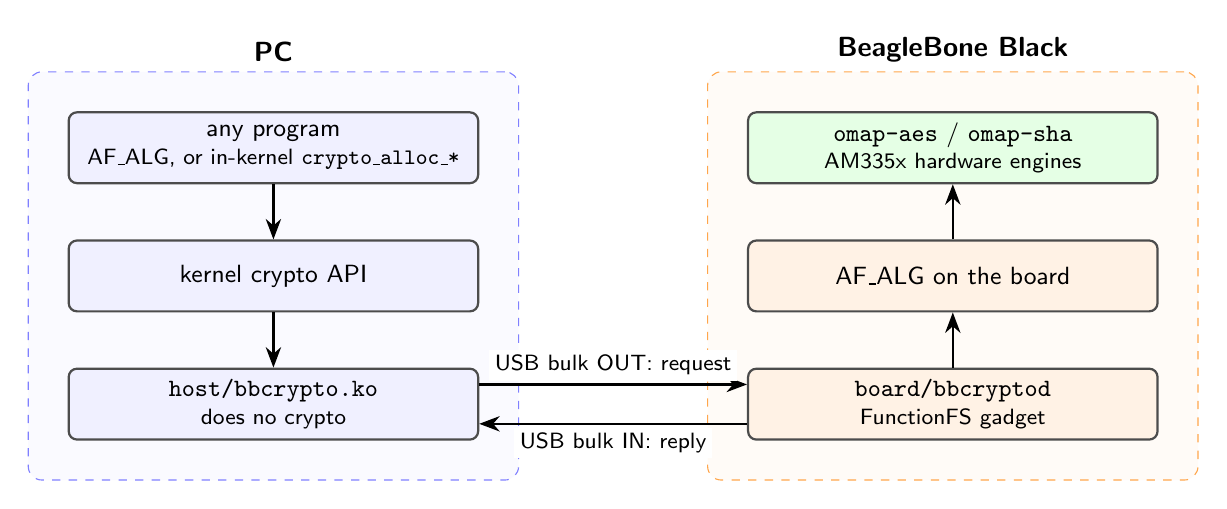
\begin{tikzpicture}[
  font=\sffamily\small,
  box/.style={draw=black!70,rounded corners=3pt,thick,align=center,minimum height=9mm,minimum width=52mm,fill=white},
  host/.style={box,fill=blue!6},
  board/.style={box,fill=orange!10},
  hw/.style={box,fill=green!10},
  flow/.style={-{Stealth[length=2.6mm]},thick},
  lab/.style={font=\sffamily\footnotesize,fill=white,inner sep=2pt}
]
\node[host] (app) {any program\\[-1pt]{\footnotesize AF\_ALG, or in-kernel \texttt{crypto\_alloc\_*}}};
\node[host,below=7mm of app] (api) {kernel crypto API};
\node[host,below=7mm of api] (mod) {\texttt{host/bbcrypto.ko}\\[-1pt]{\footnotesize does no crypto}};

\node[board,right=34mm of mod] (d) {\texttt{board/bbcryptod}\\[-1pt]{\footnotesize FunctionFS gadget}};
\node[board,above=7mm of d] (alg) {AF\_ALG on the board};
\node[hw,above=7mm of alg] (hw) {\texttt{omap-aes} / \texttt{omap-sha}\\[-1pt]{\footnotesize AM335x hardware engines}};

\draw[flow] (app) -- (api);
\draw[flow] (api) -- (mod);
\draw[flow] ($(mod.east)+(0,2.5mm)$) -- node[lab,above=1pt]{USB bulk OUT: request} ($(d.west)+(0,2.5mm)$);
\draw[flow] ($(d.west)-(0,2.5mm)$) -- node[lab,below=1pt]{USB bulk IN: reply} ($(mod.east)-(0,2.5mm)$);
\draw[flow] (d) -- (alg);
\draw[flow] (alg) -- (hw);

\begin{scope}[on background layer]
  \node[draw=blue!50,dashed,rounded corners=5pt,fill=blue!2,fit=(app)(api)(mod),inner sep=5mm,
        label={[font=\sffamily\bfseries]above:PC}] {};
  \node[draw=orange!70,dashed,rounded corners=5pt,fill=orange!3,fit=(hw)(alg)(d),inner sep=5mm,
        label={[font=\sffamily\bfseries]above:BeagleBone Black}] {};
\end{scope}
\end{tikzpicture}
\end{document}
